\section{Hegesztés, szegkötés}

%{{{ Hegesztés
\subsection{Hegesztés}

\begin{wrapfigure}{R}{.5\textwidth}
	\centering
	\vspace{-2cm}
	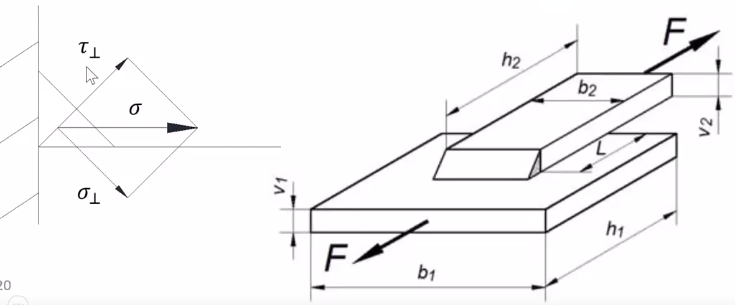
\includegraphics[width=\linewidth, trim=0 4 0 0, clip]{sarokvarrat}
	\caption{Sarokvarrat}
\end{wrapfigure}
\parbox{.49\textwidth}{
\begin{outline}
	\1 adatok
		\2 $F = 75$ kN
		\2 $\sigma_\text{meg} = 80$ MPa
		\2 $b_1 = 200$ mm, $b_2 = 100$ mm
		\2 $h_1 = 300$ mm, $h_2 = 200$ mm
		\2 $v_1 = 15$ mm, $v_2 = 18$ mm
		\2 $L = 125$ mm
\end{outline}}
\begin{outline}
	\1 megoldás
		\2 fő igénybevétel húzás
		\2 varrat gyökmérete $a = \frac{\sqrt{2}}{2}v_2 = 12.73$ mm
		\2 varrat keresztmetszete $A = a(b_2 - 2a) = 949~\text{mm}^2$
		\2 feszültség $\sigma = \frac{F}{A} = 79$ MPa
		\2 $\sigma_\perp = \tau_\perp = 55.9$ MPa
		\2 $\sigma_\text{ö} \sqrt{\sigma_\perp^2 + \sigma_\parallel^2 - \sigma_\perp\sigma_\parallel + 3\brc{\tau_\perp^2+\tau_\parallel^2}} = \sqrt{\sigma_\perp^2 + 3\tau_\perp^2} = 111.8$ MPa
		\2 $\sigma<\sigma_\text{meg}\Rightarrow$ nem felel meg
		\2 anyagot, jóságtényezőt lehet változtatni
\end{outline}

%}}}

%{{{ Szegkötés
\subsection{Szegkötés}

\begin{wrapfigure}{R}{.4\textwidth}
	\centering
	\vspace{-4cm}
	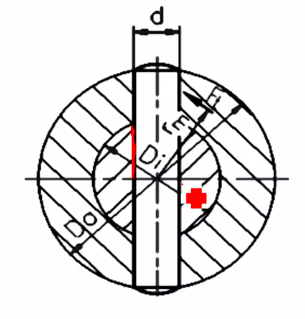
\includegraphics[width=\linewidth, trim=0 4 0 0, clip]{szegkotes}
	\caption{Szegkötés}
\end{wrapfigure}

\parbox{.49\textwidth}{
\begin{outline}
	\1 adatok
		\2 $d = 8$ mm
		\2 $D_\text{a} = 60$ mm
		\2 $D_\text{i} = 30$ mm
		\2 szeg megengedett feszültségei
			\3 $\tau_\text{max} = 95$ MPa
			\3 $p_\text{max} = 190$ MPa
		\2 tengelyre megengedett csúsztatófeszültség $360$ MPa
		\2 kibírja-e a kötés a 450 Nm-es csavaró nyomatékot?
\end{outline}}
\begin{outline}
	\1 megoldás
		\2 nyírás
			\3 $F_\tau = \frac{M_\text{t}}{\frac{D_\text{t}}{2}} = 30$ N
			\3 $A_\tau = \frac{2d^2\pi}{4} = 100.6~\text{mm}^2$
			\3 $\tau_\text{v} = \frac{F_\tau}{A_\tau} = 298$ MPa $ > \tau_\text{meg}$
			\3 nyírásra nem felel meg
		\2 felületi nyomás 1
			\3 $F_\text{p1} = \frac{M_\text{t}}{\frac{D_\text{i}+D_\text{a}}{4}} = 20$ kN
			\3 $A_\text{p1} = 2\frac{D_\text{a}-D_\text{i}}{4}d = 240~\text{mm}^2$
			\3 $p_1 = \frac{F_\text{p1}}{A_\text{p1}} = 83.3$ MPa $ < p_\text{meg}$
			\3 megfelel
		\2 felületi nyomás 2
			\3 $F_\text{p2} = \frac{M_\text{t}}{\frac{D_\text{i}+D_\text{a}}{4}} = 60$ kN
			\3 $A_\text{p2} = 2\frac{D_\text{a}-D_\text{i}}{4}d = 240~\text{mm}^2$
			\3 $p_2 = \frac{F_\text{p2}}{A_\text{p2}} = 250$ MPa $ > p_\text{meg}$
			\3 nem felel meg
		\2 vagy méreteket kell növelni, vagy erősebb anyagot választani
		\2 különlegességek
			\3 tengely poláris másodrendű nyomatéka $I_\text{p} = \frac{D_\text{i}^2\pi}{32} = 7.95\cdot10^{-8}~\text{m}^4$
			\3 $\tau = \frac{M_\text{t}}{I_\text{p}}e = 84.9$ MPa $ < \tau_\text{meg}$
			\3 ha közel van a határértékhez, $I_\text{p}$-nél nem hanyagolhatjuk el a kivágást
\end{outline}

%}}}
